\documentclass[12pt]{article}
\usepackage{amsmath}
\usepackage{amssymb}
\usepackage{listings}
\usepackage{graphicx}
\usepackage{nopageno}
\usepackage{color}

\definecolor{listingbg}{rgb}{0.99, 0.96, 1}
\definecolor{commentbg}{rgb}{0.3, 0.3, 0.8}
\lstloadlanguages{Haskell}
\lstnewenvironment{code}
    {\lstset{}%
      \csname lst@SetFirstLabel\endcsname}
    {\csname lst@SaveFirstLabel\endcsname}
    \lstset{
      language=Haskell,
      basicstyle=\footnotesize,
      flexiblecolumns=false,
      basewidth={0.5em,0.45em},
      sensitive=true,
      numberstyle=\tiny,
      numberblanklines=true,
      literate={+}{{$+$}}1 {/}{{$/$}}1 {*}{{$*$}}1 {=}{{$=$}}1
               {>}{{$>$}}1 {<}{{$<$}}1 {\\}{{$\lambda$}}1
               {\\\\}{{\char`\\\char`\\}}1
               {->}{{$\rightarrow$}}2 {>=}{{$\geq$}}2 {<-}{{$\leftarrow$}}2
               {<=}{{$\leq$}}2 {=>}{{$\Rightarrow$}}2 
               {\ .}{{$\circ$}}2 {\ .\ }{{$\circ$}}2
               {>>}{{>>}}2 {>>=}{{>>=}}2
               {|}{{$\mid$}}1               
    }

\DeclareMathOperator*{\argmax}{arg\,max}
\DeclareMathOperator*{\Merge}{Merge}

\renewcommand{\Pr}[1]{\ensuremath{\mathrm{Pr}\{ #1 \}}}

\begin{document}
\frenchspacing

\author{Joseph Abrahamson}
\title{520.666: Project \#3}

\maketitle

\section{Agglomerative letter clustering}
\label{sec:agg}

One kind of entropy-justified tree can be grown from the bottom up by
merging sets of objects such that each merge is between the two sets
with the largest mutual information. If you have a set of elements
$\mathcal{A} \triangleq \{a_i\}_{i = 0}^N$, then you can begin with
$\mathcal{S}_0 \triangleq \{s_i = \{a\} : a \in \mathcal{A}\}$ and
perform the merge $\Merge_{0 \to 1}(i, j) \implies \mathcal{S}_1 =
\Merge_{0 \to 1}(i, j)(\mathcal{S}_0) = \mathcal{S}_0\backslash\{s_i,
s_j\} \cup \{(s_i \cup s_j)\}$. We then define the algorithm as the
sequential application of the $(N-1)$ merges $$\Merge_{0\to1},
\Merge_{1\to2}, ... \Merge_{(N-1)\to N}$$ such that each merge
satisfies
\begin{align}
  \Merge_{k\to(k+1)}(i, j) : (s_i, s_j) = \argmax_{\Merge(i, j) : s_i, s_j \in \mathcal{S}_k}
    I(\Merge(i, j)(\mathcal{S}_k))
\end{align}
where
\begin{align}
  I(\mathcal{S}_k) &\triangleq \sum_{l, m : s_l, s_m \in \mathcal{S}_k} f(s_l,
  s_m) \log\frac{f(s_l, s_m)}{f(s_l) f(s_m)} \\
  f(s) &\triangleq \sum_{a \in s} f(a) \\
  f(s_l, s_m) &\triangleq \sum_{a_l \in s_l} \sum_{a_m \in s_m} f(a_l, a_m)
\end{align}
and the unigram and bigram frequencies are defined on the original
atomic set $f(a) = f(\langle a \rangle)$ and $f(a_i, a_j) = f(\langle
a_i a_j\rangle)$. Note that since each merge operation reduces the
number of sets in $\mathcal{S}_k$ by 1, $|\mathcal{S}_k| = N-k$,
$\mathcal{S}_{(N-1)} = \{\mathcal{A}\}$ providing a
simple count for how many operations need to be performed.

This recursive pairing behavior leads naturally the construction of a
tree with the atoms in $\mathcal{A}$ at the leaves and also implies
that if you split the full tree into two haves starting at the root
node then the two sets containing the atoms from the left and right
halves will have a small mutual information $I$ value, though it is
not clear that it is the smallest possible split.

\subsection{Experimental results}

Performing this sort of agglomerative clustering over a set of atoms
defined as the 26 English letters plus space \texttt{' '} formed an
agglomerative tree (displayed in Figure
\ref{fig:agglomerative-bubbles}). This tree demonstrates similar
entropic properties of English letters as an HMM model of English text
in that the first-grouping (derived by splitting the tree at the root
node) separates the atoms into the set of ``vowels $+$ space'' and
``consonants'' which corresponds to the two-state HMM model's emission
densities. The second-grouping (derived by performing a first-grouping
on each of the above sets) produces the 4 sets (\texttt{'aoiue'},
\texttt{' '}, \texttt{'rxlnsydg'}, \texttt{'vzkmfjqbpcwth'}) which
clearly splits the space from the vowels and splits consonants into
two groups. This corresponds in part to the 4-state HMM model's
emission densities, although the consonant breakdown was different.

\begin{figure}
  \centering
  \makebox[\textwidth]{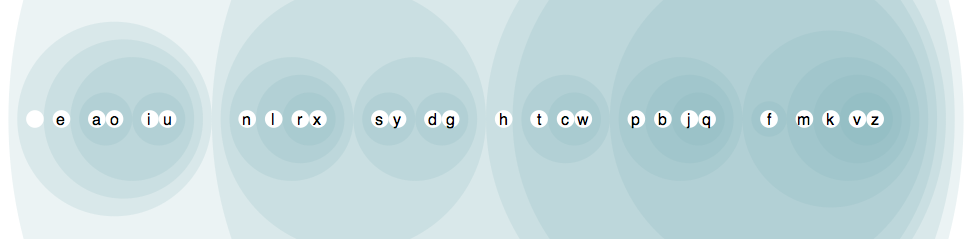
\includegraphics[width=7in]{agglomerative-bubbles}}
  \caption{\textbf{Agglomerative clustering of English letters on a
      training text leads to this letter grouping tree.} Grey circles
    are drawn such that at any particular level in the hierarchy,
    atoms contained within the circle are clustered together. Thus,
    smaller circles imply groupings closer to the leaves (with the
    leaves displayed in white) and larger circles are sets closer the
    the root of the tree.}
\label{fig:agglomerative-bubbles}
\end{figure}

\section{Bitstring encoded decision trees}

Using the bottom-up method of agglomerative clustering from section
\ref{sec:agg} we can generate a string of binary predictors of any
atom $a \in \mathcal{A}$ from the path between the root node and that
particular atom. Such bitstrings can be encoded such as
$\langle$LLRLRRLRR$\rangle$ and unambiguously select a particular
atom. Moreover, any left substring of a predictor of this form will
denote the subset of $\mathcal{A}$ that both contains $a$ and has the
maximual mutual information with $a$. In this way we can guarantee
that if an actor interested in predicting $a$ knew some left substring
of $a$'s bitstring encoding, the best next question for that actor to
ask would be the leftmost unseen ``bit'' in the string.

This leads directly to a sensible algorithm for decision tree growth
by suggesting a choice of best possible questions at each node. In
particular, for a model with $n$ predictors, moving through the
decision tree should be an exercise of walking down the paths in the
agglomerative tree leading to each of the $n$ predictors
independently, one question at a time. At any node in the decision
tree, you pick one of $n$ questions depending on which predictor will
provide the most information about the predicted quantity when we
learn one more bit about it.

So with that set of admissible questions, we greedily build a decision
tree, recursively picking the best possible question of the $n$
admissible ones by measure of the lowest post-split entropy on the
predictor. This means that if in a particular node we have limited the
admissible conditionals to a set $M$, and after asking a question $q$
this is split into the disjoint sets $M_{q^+}$ and $M_{q^-}$, we
search for the $q$ such that
\begin{align}
  \arg\min_q \left\{ \frac{|M_{q^+}|}{|M|}H(x | x \in M_{q^+}) +
  \frac{|M_{q^-}|}{|M|}H(x | x \in M_{q^-})\right\} \label{node-entropy}
\end{align}

Note that different from the algorithm advised, here we choose $q$
conditional only locally to the node we're considering splitting. This
is because the $q$ which is the minimizer of \eqref{node-entropy} will
be that maximizer invariant of the state of the rest of the tree and
thus we do not need to compute the global entropy given each possible
$q$, just the local entropy.

The stopping criterion for this tree involves the computation of the
same entropy measures on a held-out set of data. So long as the
entropy change induced by a split is greater in magnitude than a
certain cutoff (0.005 bits in this case), the split induced by entropy
minimizer question $q$ is accepted as a new branching node in the
decision tree. If the held out entropy change is not larger than that
cutoff, however, that node is barred from splitting further.

By structuring the tree growth algorithm like this (most importantly
noting the locality of the $q$ minimizer condition) an elegant
recursive algorithm can be performed (Haskell pseudocode)

\begin{code}
buildDTree :: ([Obs], [Obs]) -> (Double, Double) -> QList -> DTree Question ()
buildDTree (dev, ho) (h_dev, h_ho) qlist = 
  if h_ho - h_ho' > reductionThreshold
  then Branch bestQ (buildDTree (dev_left, ho_left) (h_dev', h_ho') qlst')
                    (buildDTree (dev_right, ho_right) (h_dev', h_ho') qlst')
  else Leaf ()
  where
    h_ho'  = splitEntropy ho bestQ
    h_dev' = splitEntropy dev bestQ
    (dev_left, dev_right) = splitByQuestion dev bestQ
    (ho_left, ho_right) = splitByQuestion ho bestQ
    (bestQ, qlist') = minimumBy (comparing (splitEntropy dev)) qlist
\end{code}

where each node either generates a new branch or terminates and the
children of the new branches are recursively generated by the same
procedure.

\subsection{Experimental results}

Using the same training text that, in whole, generated the
agglomerative tree over English letters, to generate a 4-gram
prediction task of English spelling, a decision tree was generated
according to the above algorithm. This involved searching through a
list of 3 questions at each potential branching decision, one for each
history letter. The final tree has 270 fully-specified ``leaf''
distributions corresponding to a complete partitioning of the trigram
histories into 270 fine-grained equivalence classes.

Various representations of the questions asked in the tree are shown
in Figures \ref{fig:bs_wedges}, \ref{fig:bs_examplepaths},
\ref{fig:bs_jumpcounts}. In particular, from Figure
\ref{fig:bs_wedges} it is clear that the algorithm both,
interestingly, clarifies the skip character first, but does not ask
the maximum number of questions (9) of it before moving on to
clarifying others. It also shows paths ranging between 5 and 10
questions in length.

Figure \ref{fig:bs_examplepaths} gives concrete examples of many
paths, which quickly group visually into paths which tend to clarify
characters one by one (smoothly moving black lines) versus paths which
rapidly oscillate between clarifing two character simultaneously
(oscillating paths). It also again serves to demonstrate the variation
in path length in the tree.

Figure \ref{fig:bs_jumpcounts} is a transition frequency matrix
between various questions and demonstrates with its strong 1st
superdiagonal that once a character is queried, it tends to be further
clarified (especially $w3$, the word directly preceeding the predicted
character).

While the decition tree here was trained on a text of 30k characters,
a 5k letter test text was retained. Model perplexity was measured at
10.12 on this test text which represents an improvement of 6.91 over a
unigram model. In order to compute this perplexity, a smoothing method
was needed since many of the leaf equivalence classes had no examples
of particular characters in the training text. The backoff method used
was chosen for simplicity of implementation, and only involved backing
up the tree until one of the frequency estimates was non-zero and
using that as the tree's prediction.


\begin{figure}
  \centering
  \makebox[\textwidth]{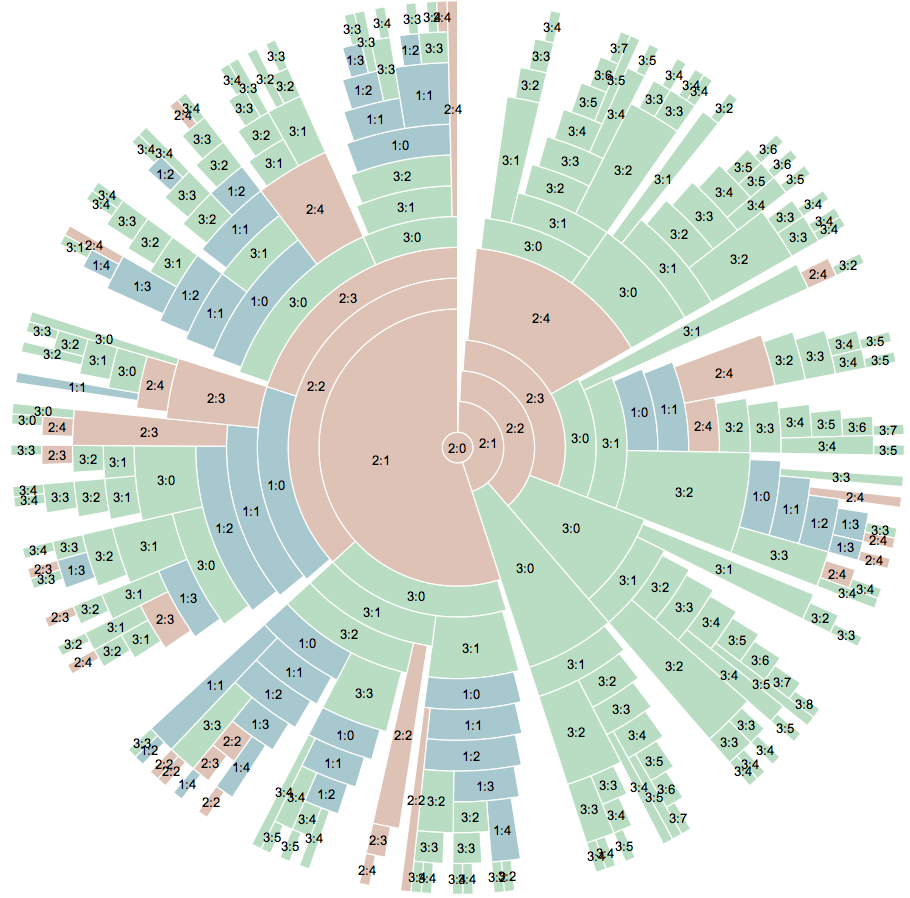
\includegraphics[width=7.5in]{bs_wedges}}
  \caption{\textbf{A representation of the bitstring question grown
      decision tree for English spelling.} Here the root node is
    represented as the circle in the center with each label $x:y$
    meaning that the predictive question asked at that node was of the
    $y$th most informative bit of the $x$th word (with strings labeled
    $\langle w_1 w_2 w_3 w_4 \rangle$ and $w_4$ being
    predicted). Additionally, each node's wedge is colored to
    correspond with the word being queried.}
  \label{fig:bs_wedges}
\end{figure}

\begin{figure}
  \centering
  \vspace{-1in}
  \makebox[\textwidth]{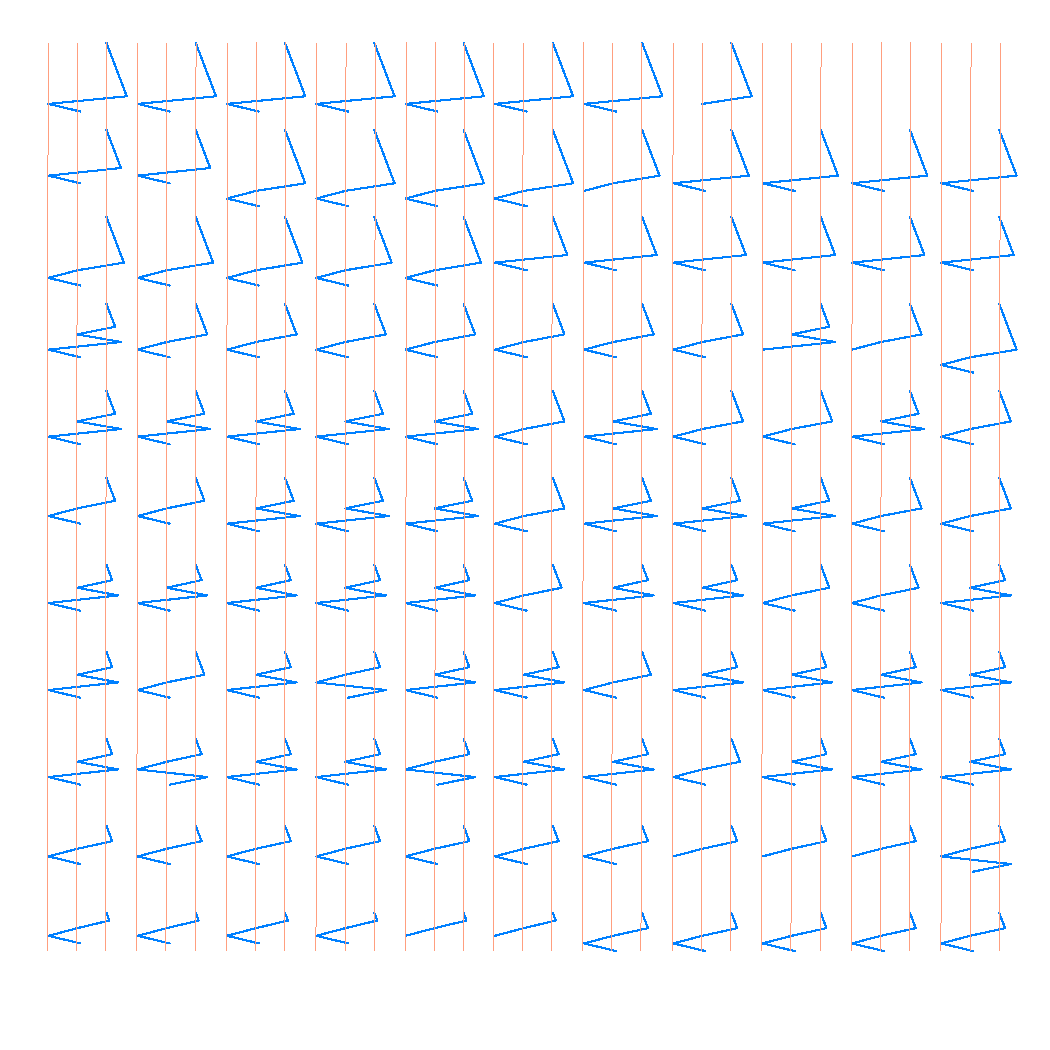
\includegraphics[width=7in]{bs_path_270}}
  \caption{\textbf{All 270 ``question paths'' extracted from the
      experimental decision tree.} The $x$-axis in each small multiple
    plot corresponds to an index into the concatenated bitstring
    $\langle b_1 b_2 b_3 \rangle$ where $b_i$ is the bitstring
    corresponding to $w_i$ in the observed 4-gram $\langle w_1 w_2 w_3
    w_4 \rangle$. The multiples are ordered from the leftmost path
    ($\langle$LLLLL $...\rangle$) in the lower left corner to the
    rightmost in the upper right and varies minimally from its
    horizontal neighbors. Each black line then traces the questions
    asked on a random walk through the decision tree while the red
    lines denote character boundaries in the concatenated bitstring.}
  \label{fig:bs_examplepaths}
\end{figure}

\begin{figure}
  \centering
  \makebox[\textwidth]{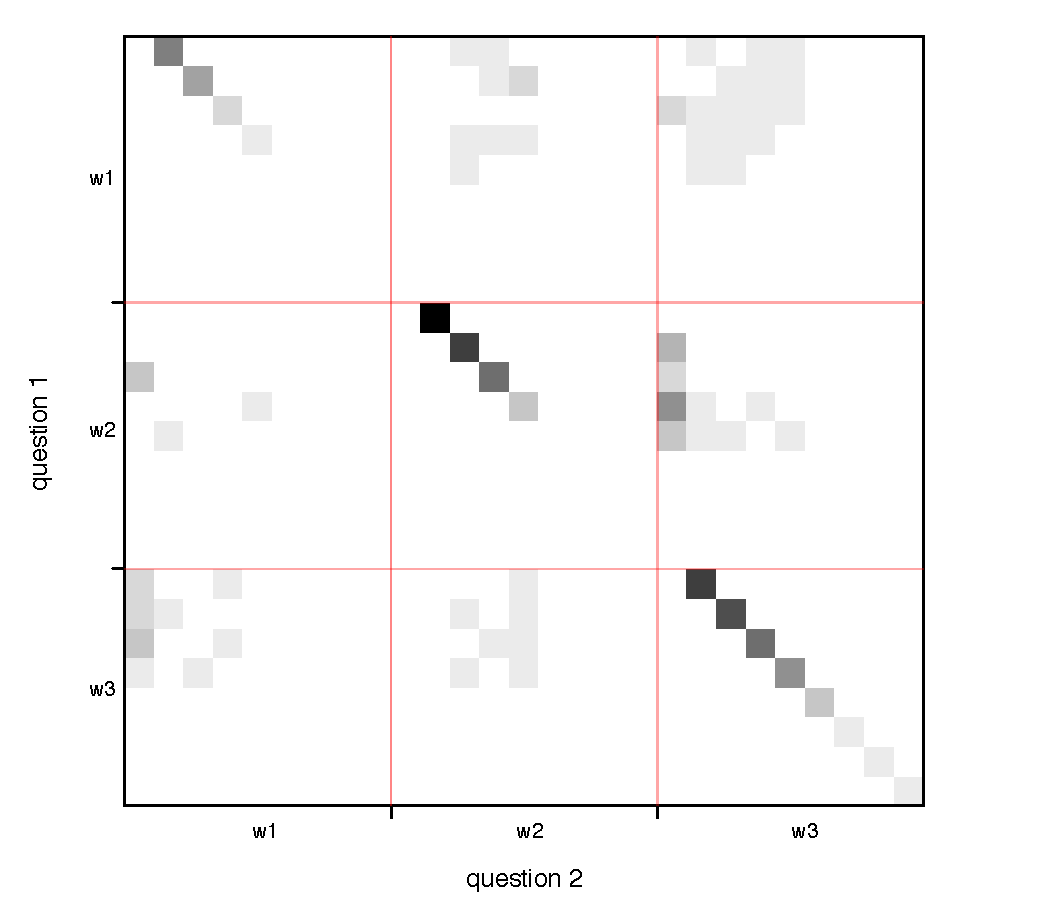
\includegraphics[width=4in]{bs_jumpcounts}}
  \caption{\textbf{Question pair frequencies in the experimental
      decision tree.} Here the $x$ and $y$ axes represent indices into
    the concatenated predictive bitstring (see Figure
    \ref{fig:bs_examplepaths}) and the colored bins represent pairs of
    questions such that the $x$-axis question was asked after the
    $y$-axis question and darker colors are more frequently observed
    pairs across all paths in the decision tree.}
  \label{fig:bs_jumpcounts}
\end{figure}

\end{document}